\chapter{Một số lớp lỗ hổng bảo mật trên ứng dụng web}
% TODO: mô tả thêm những hướng có thể dựa trên background ở trên nhưng chỉ tập trung vào application layer và HTTP request/response
Trong phạm vi hiện thực công cụ, tôi chỉ tập trung vào việc tìm hiểu và phát hiện ba lỗ hổng bảo mật ở tầng ứng dụng của ứng dụng web, cụ thể là \acrfull{xss}, \acrfull{lfi} và time-based \acrlong{sqli} (SQLI). Đầu tiên, tôi sẽ trình bày về \acrfull{xss}, một trong những lỗ hổng bảo mật phổ biến nhất trên ứng dụng web, luôn góp mặt trong top 10 lỗ hổng nguy hiểm nhất theo OWASP \parencite{owasp-top-10} nhiều năm gần đây. Nội dung phần này bao gồm làm rõ khái niệm \acrshort{xss}, phân loại và phân tích các kĩ thuật phòng thủ đối với từng loại trong lớp lỗ hổng bảo mật này.
\section{Cross-Site Scripting}
\acrfull{xss} \parencite{sullivan2011web,owasp-xss,portswigger-xss,li2011survey} là lỗ hổng bảo mật trên ứng dụng web cho phép tin tặc can thiệp vào quá trình tương tác giữa người dùng với ứng dụng web mắc lỗi này. Nguyên nhân gốc rễ của \acrshort{xss} là do ứng dụng web chấp nhận hoặc hiển thị dữ liệu đầu vào nhận được mà không qua một sự xác nhận hay mã hóa (encode) nào. Lỗ hổng \acrshort{xss} khai thác sự lỏng lẻo của \acrshort{sop} vốn được thiết kế để tách bạch quyền thực thi mã giữa các website với nhau. Một trong những hệ quả thường gặp nhất khi tin tặc khai thác thành công lỗ hổng này là cookies/mật khẩu của người dùng bị đánh cắp thông qua Javascript, từ đó tin tặc có thể mạo danh người dùng thực hiện những hành động mà người dùng có quyền hạn trên các ứng dụng web mắc lỗi này, hoặc, truy cập vào những dữ liệu nhạy cảm khác của họ. Nghiêm trọng hơn, nếu người dùng bị mạo danh trên có đặc quyền cao trong ứng dụng web thì tin tặc có thể có toàn quyền kiểm soát mọi chức năng và dữ liệu của ứng dụng, dẫn đến nhiều tổn thất nặng nề. \par
Tin tặc khai thác được lỗi \acrshort{xss} có thể thao túng ứng dụng web mắc lỗi này, khiến nó trả về mã độc Javascript cho người dùng. Việc thao túng đó có thể ``vĩnh viễn'' nếu không có động thái vá lỗi và gỡ bỏ mã độc khỏi ứng dụng web của quản trị viên (đối với trường hợp stored/persistent \acrshort{xss}), hoặc chỉ ``tạm thời'' khi người dùng vừa mở trang web có lỗ hổng đồng thời với trang web chứa mã khai thác của tin tặc (đối với trường hợp reflected \acrshort{xss}). Khi mã độc đó được thực thi bởi trình duyệt web của người dùng, nó sẽ mạo danh hoặc đánh cắp dữ liệu của người dùng như đã mô tả ở phần khái niệm. Hình \ref{fig:xss-concept} sau mô tả cách thức khai thác lỗ hổng từ phía tin tặc.
\begin{figure}[H]
  \centering
    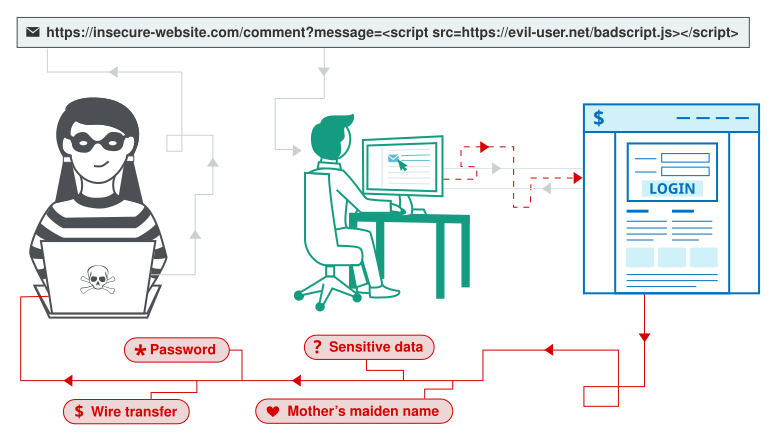
\includegraphics[width=\textwidth,keepaspectratio=true]{images/xss-concept.png}
  \caption[Mô phỏng cách thức khai thác lỗ hổng XSS]{Mô phỏng cách thức khai thác lỗ hổng \acrshort{xss} \parencite{portswigger-xss}}
  \label{fig:xss-concept}
\end{figure}
Bằng việc bypass \acrshort{sop} đối với website ``\texttt{https://insecure-website.com/}'' có lỗ hổng \acrshort{xss}, tin tặc có thể thao túng để nhúng mã độc từ một địa chỉ web khác, cụ thể là ``\texttt{https://evil-user.net/badscript.js}'' và gửi đến trình duyệt web của người dùng. Mã độc đó lúc này được thực thi ở phía người dùng và gửi về cho tin tặc những dữ liệu nhạy cảm như cookies, mật khẩu hoặc cho phép hắn mạo danh thực hiện những thao tác mà người dùng có quyền, ví dụ như chuyển khoản (wire transfer) như trong hình. Ngoài ra tin tặc còn có khả năng tấn công thay đổi giao diện (deface) trang web hoặc nhúng các đoạn mã gián điệp (trojan) tinh vi vào ứng dụng web nếu hắn khai thác thành công lỗ hổng bảo mật này. Dựa vào nguồn gốc của mã độc được trả về trình duyệt web người dùng, người ta chia lỗ hổng \acrshort{xss} thành ba loại chính: Reflected \acrshort{xss}, Stored/Persistent \acrshort{xss} và Document Object Model (\acrshort{dom}) based \acrshort{xss}, được trình bày trong các mục tiếp theo.

\subsection{Reflected XSS}
Reflected \acrshort{xss} là loại phổ biến nhất trong cả ba, nó phát sinh khi ứng dụng web có lỗi ở phía máy chủ (server-side) nhận một HTTP request chứa mã độc/payload và trả về response có chứa mã độc/payload đó cho người dùng mà không qua kiểm định sàng lọc nào từ phía máy chủ ứng dụng web. Ví dụ như trang web tìm kiếm ``\texttt{http://testphp.vulnweb.com/search.php?test=query}'' trả về kết quả tìm kiếm chuỗi ``\texttt{the}'' như trong Hình \ref{fig:vuln-web} dưới đây.
\begin{figure}[H]
  \centering
    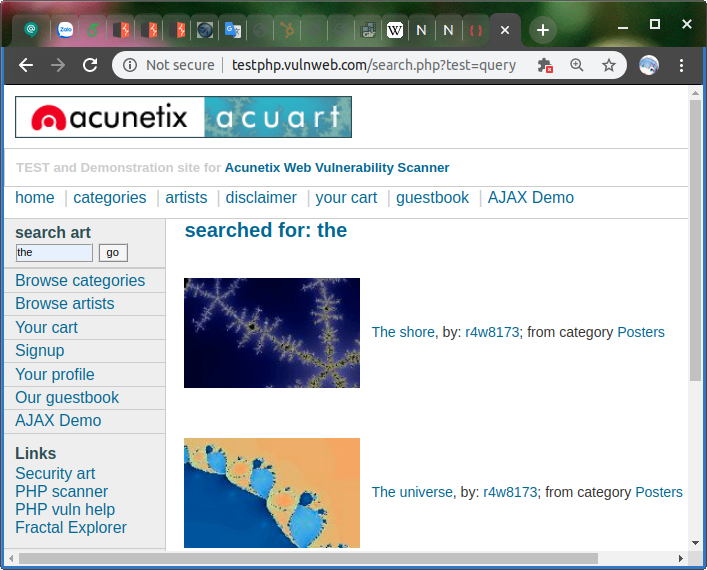
\includegraphics[width=\textwidth,keepaspectratio=true]{images/vuln-web.png}
  \caption{Ví dụ về trang web tìm kiếm có lỗ hổng Reflected XSS}
  \label{fig:vuln-web}
\end{figure}
Thay vì tìm kiếm những chuỗi kí tự bình thường, ta thử tìm kiếm với payload Javascript\\
\texttt{<script>alert('y4t0g4m1')</script>}. Kết quả trả về của trang web kết xuất thành một thông báo \texttt{alert} trên trình duyệt web như Hình \ref{fig:reflected-xss-poc}.
\begin{figure}[H]
  \centering
    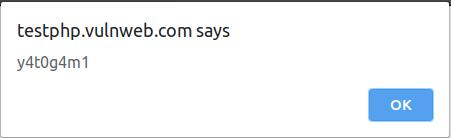
\includegraphics[width=0.6\textwidth,keepaspectratio=true]{images/reflected-xss-poc.jpg}
  \caption{Bằng chứng (\acrshort{poc}) khai thác thành công lỗ hổng XSS}
  \label{fig:reflected-xss-poc}
\end{figure}
Ví dụ trên cho thấy ứng dụng web này đã lấy payload mà ta gửi trong HTTP request trả về trong response, khiến trình duyệt web thực thi đúng đoạn mã \texttt{alert} đó, đây là lỗ hổng Reflected \acrshort{xss}. Trong thực tế, thay vì những lệnh vô hại như \texttt{alert}, tin tặc có thể thực hiện bất kì thao tác nguy hiểm nào như đánh cắp cookies và gửi về cho hắn thông qua biến \texttt{document.cookies} từ trình duyệt web của nạn nhân. Thông thường, tin tặc sẽ khai thác lỗ hổng này bằng cách dẫn dụ người dùng mở một trang web do hắn tự tạo ra cùng lúc với ứng dụng web mục tiêu, trang web tự tạo đó sẽ gửi \acrshort{http} request hoặc khiến trình duyệt web tạo và gửi request theo ý muốn của tin tặc đến ứng dụng web mục tiêu. Sau đó tin tặc đã có thể thực hiện những thao tác trên ứng dụng web mục tiêu với danh nghĩa người dùng hoặc đánh cắp dữ liệu cá nhân trên trình duyệt web của họ. Các trang web nguy hiểm do tin tặc tạo ra đó rất thường gặp trong quá trình duyệt web, nó có thể xuất hiện trong các popup, quảng cáo, hoặc trong cả email với nội dung bắt mắt nhằm giữ chân người dùng ở trang web đó càng lâu càng tốt, tùy vào phục vụ mục đích khai thác lỗ hổng của hắn. Đây là điều kiện đủ để có thể khai thác lỗ hổng \acrshort{xss} trong thực tế, người dùng sẽ không biết có sự xuất hiện của một payload đáng ngờ như \texttt{<script>alert('y4t0g4m1')</script>} đối với trường hợp trong ví dụ trên. Việc sử dụng lệnh \texttt{alert} trong payload sau đó kiểm tra xem có thông báo xuất hiện từ trình duyệt web hay không bằng công cụ \textbf{Selenium} là phương pháp phát hiện lỗ hổng \acrshort{xss} được hiện thực trong công cụ \textbf{webfuzzer} của tôi (sẽ được mô tả chi tiết trong \textbf{Chương 5}).

\subsection{Stored/Persistent XSS}
Một dạng khác trong lớp lổ hổng \acrshort{xss} là Stored/Persistent \acrshort{xss}. Tuy đều cùng là lỗi server-side nhưng khác với Reflected \acrshort{xss}, mã độc không xuất phát từ HTTP request mà từ chính ứng dụng web (thường được lưu trong cơ sở dữ liệu của ứng dụng). Lý do là vì mã độc đã được tải lên và lưu trữ trước đó thông qua HTTP request hoặc từ những nguồn không đáng tin cậy cộng với việc ứng dụng web không có cơ chế lọc hay làm sạch dữ liệu trước khi lưu trữ. Mã độc này sẽ được lưu trữ vĩnh viễn trong cơ sở dữ liệu của ứng dụng nếu không có động thái gỡ bỏ của quản trị viên. Những trang web thường mắc lỗi này bao gồm các trang bình luận của các blog, trang đăng kí và sửa đổi thông tin người dùng, các trang web trò chuyện trực tuyến, hoặc cũng có thể là một ứng dụng thư điện tử thông qua giao thức \acrshort{smtp}, một úng dụng giám sát mạng hiển thị nội dung gói tin trong đường truyền,... \par
Xét về khả năng khai thác, điểm khác biệt chính giữa Stored \acrshort{xss} và Reflected \acrshort{xss} là Stored \acrshort{xss} cho phép tin tặc lưu trữ mã khai thác và triển khai tấn công ngay trên ứng dụng web mục tiêu mà không cần phải dẫn dụ người dùng thông qua một tác nhân bên ngoài (như ví dụ ở phần Reflected \acrshort{xss}). Việc này khiến quá trình khai thác lỗi dễ dàng hơn, tin tặc chỉ việc đặt mã khai thác lên ứng dụng web và chờ đợi người dùng truy vấn đến.

\subsection{DOM-based XSS}
\acrshort{dom}-based \acrshort{xss} (hay \acrshort{dom} \acrshort{xss}) là kĩ thuật khai thác lỗ hổng \acrshort{xss} dựa trên việc thay đổi cấu trúc \acrshort{dom} của tài liệu, cụ thể là \acrshort{html}. Trong Stored \acrshort{xss} cũng như Reflected \acrshort{xss}, máy chủ ứng dụng web sẽ nhúng mã độc từ \acrshort{http} request hoặc từ cơ sở dữ liệu vào response trả về cho người dùng, hay nói cách khác hai loại này là lỗi từ phía máy chủ (server-side). Đối với \acrshort{dom}-based \acrshort{xss}, trang web ở phía người dùng (client-side) sẽ nhận mã độc và thực thi nó.\par
Dưới đây là một ví dụ về lỗ hổng \acrshort{dom}-based \acrshort{xss}. Trang web ``\texttt{http://www.vuln-web.com/user.html}'' sẽ hiển thị nội dung tùy thuộc vào tên người dùng (username) và tên người dùng này được truyền vào tham số \texttt{context} thông qua \acrshort{url}. Mã nguồn của trang \texttt{user.html} này như sau.
\begin{lstlisting}[style=htmlcssjs]
<html>
    <head>
    <title>Custom Dashboard</title>
    </head>
    This is the homepage of 
    <script>
    	var pos = document.URL.indexOf("context=") + 8;
    	document.write(document.URL.substring(pos,document.URL.length));
    </script>
</html>
\end{lstlisting}
Ví dụ, đường dẫn ``\texttt{http://www.vuln-web.com/user.html?context=John}'' sẽ đưa ta đến trang chủ của người dùng John, nội dung trang web lúc này sẽ chứa chuỗi ``\textbf{This is the homepage of John}''. Quá trình khai thác lỗi \acrshort{dom}-based \acrshort{xss} được mô tả tuần tự qua các bước sau.
\begin{enumerate}
    \item Tin tặc nhúng mã độc vào \acrshort{url}. Ví dụ\\ ``\texttt{http://www.vuln-web.com/user.html?context=<script>alert('y4t0g4m1')</script>}''.
    \item Trình duyệt web của nạn nhân nhận \acrshort{url} và tạo một \acrshort{http} request tới ``\texttt{http://www.vuln-web.com/}'', sau đó nhận về một response chứa đoạn mã \acrshort{html} tĩnh từ máy chủ.
    \item Trình duyệt web bắt đầu xây dựng \acrshort{dom} của trang web và khởi tạo thuộc tính \texttt{document.URL} trong \acrshort{url} ở bước 1.
    \item Trình duyệt phân tích đoạn mã \acrshort{html} đến đoạn mã JavaScript, nó thực thi đoạn JavaScript đó, cụ thể là trích xuất mã độc từ thuộc tính \texttt{document.URL}.
    \item Trình duyệt cập nhật nội dung \acrshort{html} của trang web dựa trên DOM đã xây dựng trước đó thành\\``\textbf{This is the homepage of <script>alert('y4t0g4m1')</script>}''
    \item Trình duyệt nhận ra đoạn mã JavaScript chứa trong cặp thẻ \texttt{<script>} và thực thi nó, làm xuất hiện thông báo \texttt{alert} khi ta truy cập vào đường dẫn ở bước 1.
\end{enumerate}
Trong thực tế, tin tặc sẽ dùng nhiều biện pháp làm rối (tampering) cũng như che giấu (obfuscating) payload để đánh lừa các bộ lọc dữ liệu đầu vào của trình duyệt web cũng như máy chủ ứng dụng web chứ không để payload lộ liễu như trong ví dụ trên. Hơn nữa mã độc hoàn toàn có thể được truyền vào ứng dụng web thông qua \acrshort{http} request nên ta cũng có thể tiến hành kiểm thử lỗi này thông qua request như đối với trường hợp Stored/Reflected \acrshort{xss}. 

\section{Local File Inclusion}
% https://www.rcesecurity.com/2017/08/from-lfi-to-rce-via-php-sessions/?fbclid=IwAR1VcA--iI7uRzwcqGk9JdcgHFZugVVNA1X2bLTSahRMhJy8Dk69gflKi8k
% https://outpost24.com/blog/from-local-file-inclusion-to-remote-code-execution-part-1
Lỗ hổng \acrfull{lfi} \parencite{portswigger-directory-traversal, owasp-path-traversal, sullivan2011web}, còn có tên khác là Path Traversal hay Directory Traversal, là lỗ hổng bảo mật trên ứng dụng web cho phép tin tặc đọc bất kì tập tin nào trên máy chủ mà ứng dụng web đang chạy trên. Những tập tin này có thể là mã nguồn, hình ảnh, dữ liệu hoặc thậm chí cả những tập tin hệ thống nhạy cảm. Trong một vài trường hợp xử lí phân quyền không tốt ở phía máy chủ, tin tặc còn có thể tạo thêm tập tin mới gây nên sự thay đổi dữ liệu và hành vi của ứng dụng, hoặc hắn có thể thực thi mã (\acrshort{rce}) từ phía máy chủ để chiếm quyền điều khiển hệ thống. Dưới đây là ví dụ về đoạn mã PHP của trang web ``\texttt{http://vuln-web.com/}'' có lỗ hổng \acrshort{lfi}.
\begin{lstlisting}[language=php]
/**
* Get the filename from a GET input
* Example - http://vuln-web.com/?file=filename.php
*/
$file = $_GET['file'];

/**
* Unsafely including the file
* Example - filename.php
*/
include('directory/' . $file);
\end{lstlisting}
Bằng cách nhận vào tham số \texttt{\$file} từ đường dẫn \acrshort{url}, máy chủ web trực tiếp trả về nội dung tập tin có tên \texttt{filename.php} trong thư mục hiện tại như trong ví dụ trên. Tin tặc có thể lợi dụng sơ hở từ câu lệnh \texttt{include('directory/' . \$file);} để trực tiếp đọc bất kì tập tin nào bằng cách sử đường dẫn tương đối, kết hợp tiền tố ``../'' (hoặc ``..\textbackslash'' đối với các máy chủ web dùng hệ điều hành Windows Server) để tham chiếu tới thư mục cha của thư mục hiện tại cộng với tên tập tin để đọc nội dung của tập tin đó, ví dụ như ``\texttt{http://vuln-web.com/?file=../../etc/passwd}''. Hình \ref{fig:lfi-payloads} sau đây minh họa một số payload dùng để đọc tập tin ``\textbf{passwd}'' trong đường dẫn \textbf{/etc/} trong các máy chủ web Unix.
\begin{figure}[H]
  \centering
    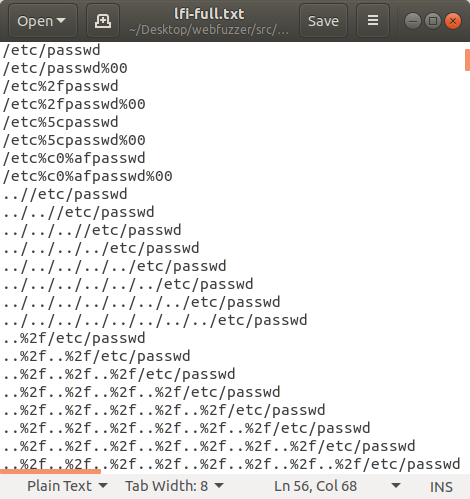
\includegraphics[width=0.7\textwidth,keepaspectratio=true]{images/lfi-payloads.png}
  \caption{Một số payload khai thác lỗ hổng \acrshort{lfi}}
  \label{fig:lfi-payloads}
\end{figure}
\textbf{/etc/passwd} là tập tin chứa danh sách tài khoản người dùng trên máy chủ web dùng hệ điều hành Unix, tập tin này bắt đầu bằng chuỗi ``\texttt{root:x}'' và chứa nhiều thông tin quan trọng như tên, địa chỉ email, đường dẫn tuyệt đối đến thư mục home trên đĩa cứng, ID của quyền (hoặc nhóm quyền) của người dùng đó,..., cung cấp cho tin tặc nhiều thông tin quý giá khi bắt đầu xâm nhập vào hệ thống. Do ta không biết độ sâu của thư mục ứng dụng web so với đường dẫn gốc (root directory) của hệ điều hành nên ta phải thử truy vấn đến từng tầng thư mục cha của thư mục hiện hành đến khi chạm tới thư mục gốc sau đó truy cập đến tập tin \textbf{/etc/passwd} như ví dụ trong Hình \ref{fig:lfi-payloads}.\par

\section{Time-based Structured Query Language Injection}
Hầu hết các kĩ thuật tấn công ứng dụng web đều tuân theo mô-típ đánh lừa ứng dụng web để thực hiện những hành động nguy hiểm thay tin tặc. Tin tặc không thể lấy được cookies của người dùng một cách chính quy nhưng có thể đánh lừa để trình duyệt web nạn nhân cung cấp cho hắn thông qua lỗ hổng \acrshort{xss}. Tin tặc cũng không thể tùy tiện truy xuất bất cứ tập tin nào trên máy chủ web nhưng hắn có thể lừa ứng dụng web làm việc đó thông qua lỗ hổng \acrshort{lfi}. Tương tự, tin tặc không thể trực tiếp truy cập và trích xuất cơ sở dữ liệu của ứng dụng web nhưng hắn có thể lừa ứng dụng web làm việc đó thông qua lỗ hổng \acrfull{sqli}. Phần này trình bày về khái niệm và các kĩ thuật phòng thủ lỗ hổng \acrshort{sqli} nói chung và time-based \acrshort{sqli} nói riêng.\par
Lỗ hổng \acrfull{sqli} \parencite{li2011survey,sullivan2011web} cho phép tin tặc can thiệp vào các câu truy vấn \acrshort{sql} mà ứng dụng web dùng để tương tác với cơ sở dữ liệu. Thông thường việc này sẽ cho phép tin tặc đọc những dữ liệu mà hắn không có quyền, ví dụ như dữ liệu của những người dùng khác trong ứng dụng hoặc kể cả những dữ liệu mà ứng dụng đó không có quyền truy cập. Trong nhiều trường hợp tin tặc còn có thể sửa đổi hoắc sao chép (dump) những dữ liệu này, gây nên rủi ro bị đánh cắp dữ liệu và những hậu quả lâu dài cho nhà cung cấp ứng dụng web. Trong một vài điều kiện đặc biệt hơn, tin tặc còn có thể leo thang một cuộc tấn công \acrshort{sqli} để thỏa hiệp máy chủ ứng dụng web đang vận hành hoặc thực hiện một cuộc tấn công \acrshort{dos}. Dưới đây là ví dụ về một đoạn mã PHP\footnote{Nguồn: http://websec.fr/level01/source.php} có lỗ hổng \acrshort{sqli}.
\begin{lstlisting}[language=php]
public function doQuery($injection) {
    $pdo = new SQLite3('database.db', SQLITE3_OPEN_READONLY);
    
    $query = 'SELECT id,username FROM users WHERE id=' . $injection . ' LIMIT 1';
    $getUsers = $pdo->query($query);
    $users = $getUsers->fetchArray(SQLITE3_ASSOC);

    if ($users) {
        return $users;
    }

    return false;
}
\end{lstlisting}
Câu truy vấn \acrshort{sql} trong ví dụ trên sẽ trả về cho người dùng giá trị của hai trường \texttt{id} và \texttt{username} của bản ghi đầu tiền trong bảng \texttt{users} có trường \texttt{id} bằng giá trị của tham số \texttt{\$injection} được truyền vào. Thông thường giá trị này thường là những chuỗi hoặc những con số có định dạng cụ thể, phục vụ cho việc truy vấn thông tin người dùng. Thông qua giao diện web hoặc \acrshort{http} request, tin tặc có thể can thiệp vào ứng dụng web và chỉnh sửa tùy ý nội dung của tham số \texttt{\$injection}. Ví dụ trong trường hợp giá trị tham số này là ``\colorbox{gray!30}{\texttt{1'; DROP TABLE users; -{}-'}}'', câu truy vấn trở thành\\
\colorbox{gray!30}{\texttt{SELECT id,username FROM users WHERE id='1'; DROP TABLE users; -{}-'}}\\
Sau khi truy vấn giá trị \texttt{id} và \texttt{username} của bản ghi có trường \texttt{id = 1} thì câu truy vấn \acrshort{sql} trên sẽ xóa toàn bộ nội dung (drop) bảng \text{users} trong cơ sở dữ liệu của ứng dụng. Bằng cách dùng dấu chấm phẩy để thực hiện nhiều câu truy vấn nối tiếp hoặc lồng nhau (nested queries), đóng mở nháy đơn và chú thích (-{}-) phù hợp với mã nguồn của trang web mà tin tặc có thể khai thác lỗ hổng \acrshort{sqli} này và gây ra hậu quả to lớn như thay đổi cấu trúc lược đồ quan hệ như ví dụ trên.\par
Lớp lỗ hổng \acrshort{sqli} có nhiều loại được phân ra dựa trên cách thức và mục tiêu tấn công \parencite{sqli-classification}, trong phạm vi luận văn này, tôi chỉ tập trung phát hiện lỗ hổng time-based \acrshort{sqli}. Time-based \acrshort{sqli} là kĩ thuật khai thác lỗ hổng \acrshort{sqli} bằng cách sử dụng những câu truy vấn đặc biệt, buộc hệ quản trị cơ sở dữ liệu phải chờ một khoảng thời gian trước khi trả về kết quả truy vấn cho ứng dụng, dựa vào thời gian phản hồi của câu truy vấn, ta có thể nhận định sự tồn tại của lỗ hổng này. Mục đích của việc kiểm thử lỗ hổng này không chỉ có vậy, việc khai thác thành công time-based \acrshort{sqli} trên những điểm cuối của một ứng dụng web còn có nghĩa là điểm cuối này cho phép truy vấn liên tiếp, lồng nhau, hoặc phát hiện được một số phần tử trong danh sách đen cũng như danh sách trắng của bộ lọc dữ liệu đầu vào, những nhận định này là cơ sở để tấn công sâu hơn vào ứng dụng web đó. Việc khai thác bằng kĩ thuật này phụ thuộc các hàm hoãn thời gian của mỗi hệ quản trị cơ sở dữ liệu khác nhau, cụ thể đối với MySQL ta dựa vào hàm ``\textbf{sleep}'' và ``\textbf{benchmark}'', đối với Microsoft SQL Server là hàm ``\textbf{waitfor delay}'' và ``\textbf{waitfor time}'', đối với Postgres SQL là ``\textbf{pg\_sleep}'',...\par
